\documentclass[11pt, a4paper]{article}
\usepackage[a4paper, margin = 0.7in]{geometry}
\usepackage{graphicx}
\usepackage{amsmath}
\usepackage{listings}
\usepackage{url}

\title{EE2703 Assignment 5 : Laplace Equation}
\author{Aman Kumar EE19B066}
\date{March 27, 2021}

\begin{document}

\maketitle

\section{The assignment}
In this assignment we do the following-
\begin{itemize}
    \item Solve for potential in a resistor.(A plate of 1$cm$ x 1$cm$ in this case)
    \item Solve for currents in that resistor.
    \item Learn to solve Laplace equation with an iterative approach and see how it converges.
    \item Learn to vectorize \textit{for} loops
\end{itemize}
\subsection{Introduction}
    A wire is soldered to the middle of a copper plate and its voltage is held at 1 Volt. One side of the plate is grounded, while the remaining are floating. The plate is 1 cm by 1 cm in size. The current density $\Vec{j}$ is related to the local Electric Field $\Vec{E}$ by the conductivity $\sigma$
    \begin{equation*}
        \Vec{j} = \sigma\Vec{E}
    \end{equation*}
    Now the Electric field is the gradient of the potential $\phi$,
    \begin{equation*}
        \Vec{E} = -\nabla\phi
    \end{equation*}
    and by continuity equation
    \begin{equation*}
        \nabla\cdot\Vec{j} = -\frac{\partial \rho}{\partial t}
    \end{equation*}
    For DC currents and a material of constant conductivity the equation becomes the Laplace equation
    \begin{equation*}
        \nabla^{2} = \phi
    \end{equation*}
    Now the Laplace equation in 2 dimensions can be written in cartesian coordinates as
    \begin{equation*}
        \frac{\partial^2 \phi}{\partial x^2} + \frac{\partial^2 \phi}{\partial y^2} = 0
    \end{equation*}
    where,
    \begin{equation*}
        {\frac{\partial \phi}{\partial x}}_{(x_i,y_j)} = \frac{\phi(x_{i + 1/2},y_j) - \phi(x_{i - 1/2},y_j)}{\Delta x}
    \end{equation*}
    so,
    \begin{equation*}
        {\frac{\partial^2 \phi}{\partial x^2}}_{(x_i,y_j)} = \frac{\phi(x_{i + 1},y_j) - 2\phi(x_i,y_j) + \phi(x_{i - 1},y_j)}{(\Delta x)^2}
    \end{equation*}
    Thus similarly we can do for $y$ as well. Since $\Delta x$ = $\Delta y$, we obtain
    \begin{equation}
        \phi_{i,j} = \frac{\phi_{i+1,j} + \phi_{i-1,j} + \phi_{i,j+1} + \phi_{i,j-1}}{4}
    \end{equation}
    which is just the average of the potentials of its neighbouring nodes(if solution holds)

\subsection{Things to do}
Mainly the following things are asked in this assignment:
    \begin{itemize}
        \item Plot the contour plot of the potential before solving(iterations) the Laplace equation. Just showing the electrode nodes at 1 V potential.
        \item Solve the Laplace equation using iterations.
        \item Plot the semilog and loglog plots of Errors(max difference) in $\phi$ after every iteration w.r.t previous iteration.
        \item Plot the 3-D surface plot of the potential after solving.
        \item Plot a contour plot of the potential after solving(iterations) the Laplace equation.
        \item Plot the vector plot of currents
        \item Plot net error vs number of iterations.
    \end{itemize}
\section{Assignment questions}
    \subsection{Defining the Parameters}
    The parameters that control the program has some default values. If the user correctly passes the required 4 arguments in the command line, then those values are accepted. Otherwise, default values are taken. Python code-
    \begin{verbatim}
if len(argv) == 5:
    Nx = min((int(argv[1]),int(argv[2])))
    Ny = min((int(argv[1]),int(argv[2])))
    if argv[1] != argv[2]:
        print("Nx and Ny should be equal for my program")
    if int(argv[3]) > Nx/2 :
        radius = 8
        print("\nRadius given is greater than size of plate. Default value is taken.")
    else:
        radius = int(argv[3])
    if int(argv[4]) > 500:
        Niter = int(argv[4])
    else:
        Niter = 1500
        print("Niter cannot be less than 500. It's default value 1500 is taken.")
else:
    print("\nUsage: %s <Nx> <Ny> <radius> <Niter>" % argv[0])    
    Nx=25
    Ny=25
    radius=8
    Niter=1500
    \end{verbatim}
    \subsection{Potential array($\phi$) initialization}
    First we initialize $\phi$ to zero and then find which nodes are in contact with the wire to make potential of nodes equal to 1 V. \textbf{numpy.where()} is used here to find the points inside the radius of wire:
    \begin{verbatim}
        phi = np.zeros((Nx,Ny))
        x = pl.linspace(0.5,-0.5,Nx)
        y = pl.linspace(0.5,-0.5,Ny)
        X,Y = pl.meshgrid(x,y)
        ii = pl.where(X*X + Y*Y <= (radius/Nx)**2)
        phi[ii] = 1
    \end{verbatim}
    Then we plot (in Figure 1) the (filled)contour plot of the intial potential using the following code(I am omitting the non-important part here):
    \begin{verbatim}
    pl.contourf(X,Y,phi)    
    pl.title("Contour Plot of Potential(2D) before solving")
    pl.scatter(X[ii],Y[ii],color="red",label="Electrode Nodes")
    pl.xlabel("X($cm$)")
    pl.ylabel("Y($cm$)")
    pl.legend()
    pl.colorbar()
    pl.show()    
    \end{verbatim}
    \subsection{Performing the Iterations}
    We use a second potential array, called \textbf{oldphi} to hold the values of the previous iteration. This is to keep track of how much the array changed during the current iteration. In this we have vectorized the \textit{for loop} so that it works with almost the speed of \textbf{C}. This is the main loop of the proagram-
    \begin{verbatim}
for k in range(Niter):
    oldphi = phi.copy()
    phi[1:-1,1:-1] = 0.25*(phi[1:-1,0:-2] + phi[1:-1,2:] + phi[:-2,1:-1] + phi[2:,1:-1])
    phi[ii] = 1

    #Boundary conditions.
    phi[1:-1,0] = phi[1:-1,1]                     #Top boundary
    phi[1:-1,-1] = phi[1:-1,-2]                   #Right boundary
    phi[0,1:-1] = phi[1,1:-1]                     #Left boundary
    phi[-1,1:-1] = 0                              #Lower boundary(grounded)
    errors[k] = abs(phi - oldphi).max()      #Finding the max change for this iteration
    \end{verbatim}
    \subsection{Plotting errors to see the convergence}
    The errors reduce but very slowly. The plot is linear in semilog. In loglog it is reasonably linear upto first 500 iterations, after that it decays exponentially. We plot every $50^{th}$ point. We fit the error to the form
    \begin{equation*}
        y = Ae^{Bx}
    \end{equation*}
    We extract the above fit for the entire vector of errors and for those error entries after the $500^{th}$ iteration. The plot of actual errors, errors using fit1 and fit2 are plotted in Figure 2 and Figure 3 for \textit{semilogy} and \textit{loglog} respectively.
    \subsection{Surface plot of potential}
    For plotting a 3-D surface plot(Figure 4) of $\phi$ the following code is used:
    \begin{verbatim}
    fig3 = pl.figure(3)
    ax=p3.Axes3D(fig3)
    pl.title("The 3-D surface plot of the potential")
    surf = ax.plot_surface(X,Y, phi, rstride=1, cstride=1, cmap=pl.cm.jet,linewidth=1)
    pl.xlabel("$x(cm)$")
    pl.ylabel("$y(cm)$")
    pl.show()        
    \end{verbatim}
    \subsection{Contour Plot of the Potential}
    This contour plot(Figure 5) is after the iteations are done. i.e. The solution for potential in the resistive plate. Python code:
    \begin{verbatim}
    fig4 = pl.figure(4)
    pl.contourf(X,Y,phi)    
    pl.title("Contour Plot of Potential(2D) after solving")
    pl.scatter(X[ii],Y[ii],color="red",label="Electrode Nodes")
    pl.xlabel("X($cm$)")
    pl.ylabel("Y($cm$)")
    pl.legend()
    pl.colorbar()
    pl.show()
    \end{verbatim}
    \subsection{Vector Plot of Currents}
    For obtaining the currents we need to compute gradient of potential $\phi$. Since the actual value of conductivity $\sigma$ does not matter to the shape of the current profile, so we set it to unity.
    \begin{equation*}
        j_x = -\frac{\partial \phi}{\partial x}
    \end{equation*}
    \begin{equation*}
        j_y = -\frac{\partial \phi}{\partial y}
    \end{equation*}
    Numerically,
    \begin{equation*}
        J_{x,ij} = \frac{\phi_{i,j-1} - \phi_{i,j+1}}{2}
    \end{equation*}
    \begin{equation*}
        J_{y,ij} = \frac{\phi_{i-1,j} - \phi_{i+1,j}}{2}
    \end{equation*}
    $\Vec{J}$ is plotted using \textit{pylab.quiver()} in Figure 6 as follows:
    \begin{verbatim}
    #Arrays to store the x and y component of currents
    Jx = np.zeros((Nx,Ny))
    Jy = np.zeros((Nx,Ny))
    
    #Calculating vector current density components
    Jx = -0.5*(phi[1:-1,:-2] - phi[1:-1,2:])
    Jy = -0.5*(phi[:-2,1:-1] - phi[2:,1:-1])
    
    #Plotting the vector Plot of Currents
    fig5 = pl.figure(5)
    pl.quiver(X[1:-1,1:-1],Y[1:-1,1:-1],Jx,Jy)
    pl.scatter(X[ii],Y[ii],color="red")
    pl.title("The vector plot of the current flow")
    pl.xlabel("X($cm$)")
    pl.ylabel("Y($cm$)")
    pl.show()
    \end{verbatim}
    \subsection{Net error vs number of iterations}
    The maximum error scales as
    \begin{equation*}
        error_k = Ae^{Bx}
    \end{equation*}
    where k is the iteration number. For the default case, I got
    \begin{equation*}
        error_k = 0.021525\exp(-0.01295k)
    \end{equation*}
    Summing up the errors, we have
    \begin{equation*}
        netError < -\frac{A}{B}exp(B(N + 0.5))
    \end{equation*}
    Thus, using this relation and our estimated values of $A$ and $B$ we plot(Figure 7) netError vs N(number of iterations). From $N = 500$ to $N = 2Niter$. Python code for doing that:
    \begin{verbatim}
    def net_error(A,B):
        return ((-A/B)*np.exp(B*(iter_ + 0.5)))
    
    NetError = net_error(A,B)
    fig6 = pl.figure(6)
    pl.semilogy(iter_,NetError,'ro',linestyle='dashed',linewidth=1,label='Net Error')
    pl.title("Net Error vs Number of iterations")
    pl.xlabel("Niter")
    pl.ylabel("Net errror")
    pl.legend()
    pl.grid(True)
    pl.show()
    \end{verbatim}
\section{Plots and Results}
    \subsection{Initial potential}
    \begin{figure}[!h]
        \centering
        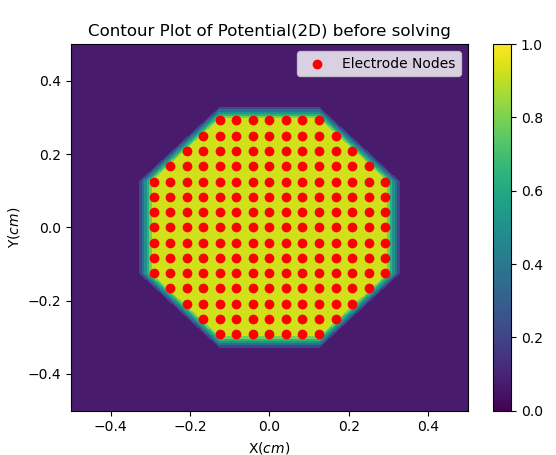
\includegraphics[scale = 0.7]{Figure1.png}
        \caption{Initial potential}
        \label{fig:Figure }
    \end{figure}
    This plot is before solving the Laplace equation. Red dots denote the nodes in contact with the electrode.They are at 1 V.
    \subsection{Errors}
    \begin{figure}[!h]
        \centering
        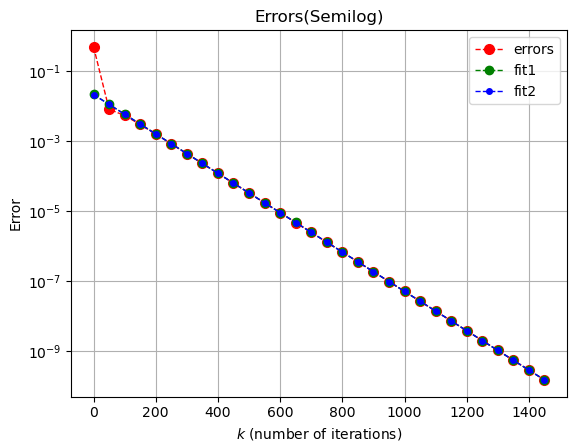
\includegraphics[scale=0.85]{Figure2.png}
        \caption{Errors on semilog}
        \label{fig:Figure 2l}
    \end{figure}
    \textit{errors} are the actual errors, while \textit{fit1} is the fit that we got by taking the entire error vector, and fit 2 is what we got from taking error entries after the $500^{th}$ point.
    \begin{figure}[!h]
        \centering
        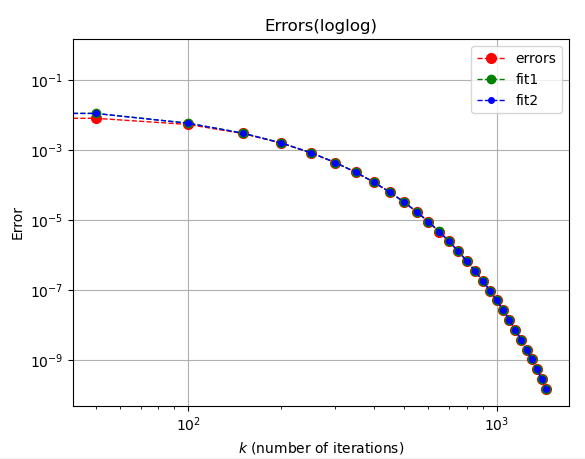
\includegraphics[scale=0.85]{Figure3.png}
        \caption{Errors on loglog}
        \label{fig:Figure 3}
    \end{figure}
    We can see that error is linear on semilog scale. In loglog scale it is linear initially but then it enters the exponential regime.
    \subsection{Potential after solving}
    \begin{figure}[!h]
        \centering
        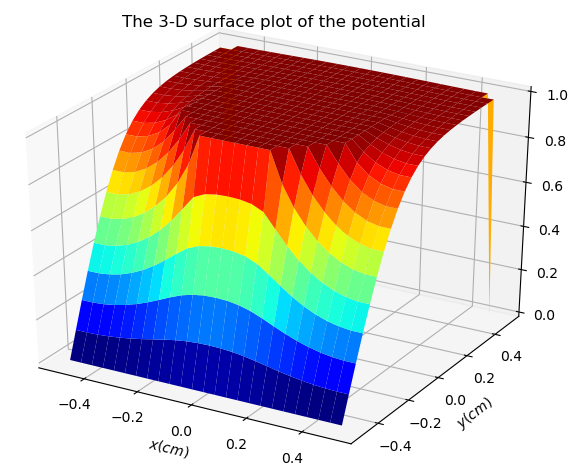
\includegraphics[scale = 0.8]{Figure4.png}
        \caption{3-D surface plot of potential}
        \label{fig:Figure 4}
    \end{figure}
    We can see the from the plot that potential is higher on the top of the plate and reduces to zero till bottom. Also since the electrode is connected to the centre of the plate, it is 1 V in the central region within the radius. Thus we expect that the current will flow from the central region to the bottom of the resistor. It will disperse a little in the middle.
    \begin{figure}[!h]
        \centering
        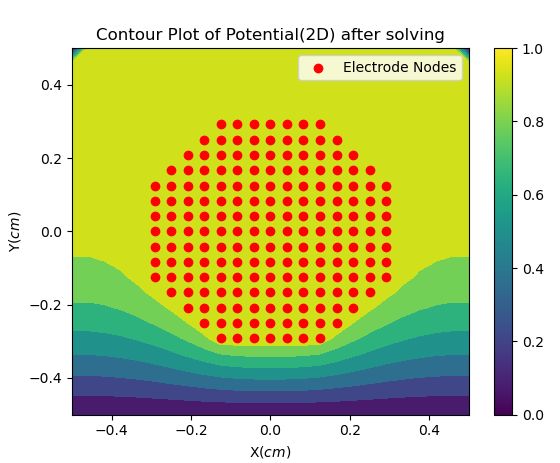
\includegraphics[scale = 0.8]{Figure5.png}
        \caption{Contour plot of Plotential}
        \label{fig:Figure 5}
    \end{figure}
    \subsection{Currents}
    \begin{figure}[!h]
        \centering
        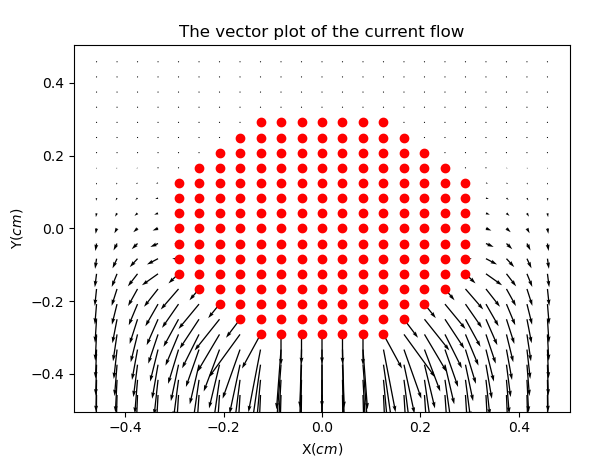
\includegraphics[scale = 0.8]{Figure6.png}
        \caption{Vector plot of currents}
        \label{fig:Figure 6}
    \end{figure}
    Thus as expected, current flows from the central region to the bottom of the resistor. It disperses a little in the middle. The part of the current directly below the central region carries major part of the current. As a result heating will be more in this region. While the top edge won't heat much.
    \subsection{Net error vs Number of iterations}
    \begin{figure}[!h]
        \centering
        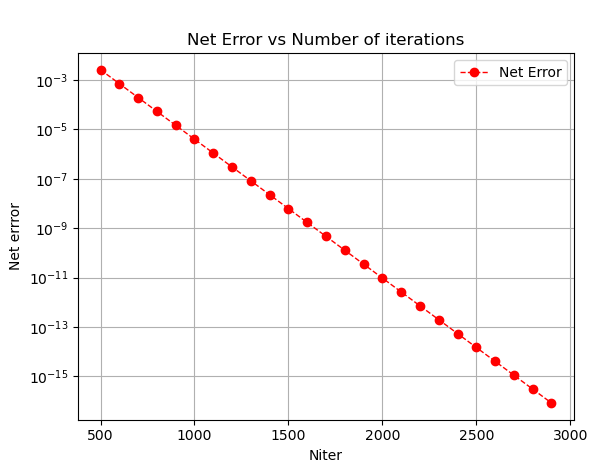
\includegraphics[scale = 0.8]{Figure7.png}
        \caption{Net error vs iterations}
        \label{fig:Figure 7}
    \end{figure}
    The net error reduces with the increase in number of iterations as expected. The semilog plot is linear which means that as the number of iterations increase the decrease in error becomes slower and slower.
\section{Conclusions}
\begin{itemize}
    \item A mojor part of the current flows only in the narrow region at the bottom.
    \item Almost no current flows in the top part of the resistive plate.
    \item To reduce the error, we have to given large values of \textit{Niter}, \textit{Nx} and \textit{Ny} to get results with better accuracy.
    \item This method of solving Laplace equations is very very slow as even after vectorizing almost all the \textit{for} loops, the program is a bit slow.
\end{itemize}
\end{document}

